\documentclass[10pt]{article}
\usepackage{palatino}
\usepackage{fullpage}
\usepackage{latexsym}
\usepackage{amsfonts}
\usepackage{hyperref}
\usepackage{multicol}
\usepackage{fancyhdr}
\usepackage{enumitem}
\usepackage{caption}
\usepackage{subcaption}
\usepackage{fancybox}
\usepackage{framed}

\pagestyle{empty}                       %no page numbers
\thispagestyle{empty}                   %removes first page number
\setlength{\parindent}{0in}

\usepackage{fullpage}
\usepackage[tmargin = 0.5in, bmargin = 1in, hmargin = 1in]{geometry}     %1-inch margins
\geometry{letterpaper}
\usepackage{graphicx}
\usepackage{amssymb}

	\thispagestyle{empty}
	\renewcommand{\headrulewidth}{0.0pt}
	\thispagestyle{fancy}
	\lhead{Name: \underline{\hspace{1.5in}}}
	\chead{MTH 201: Calculus}
	\rhead{\framebox{\textbf{Grade: \ S \quad P}} }
	\lfoot{}
	\cfoot{}
	\rfoot{}


\begin{document}

	\vspace*{0in}

		\begin{center}
			\textbf{Learning Target C3 \\
			Version 4} \\
		\end{center}


\begin{framed}
	\textbf{C3: Interpret or apply information about a function and its first two derivatives; or, draw conclusions about a function and its first two derivatives given information about the function. }
\end{framed}

Below is the graph of a function $y = f(x)$, which is defined on the interval $[-4,4]$. The units of $x$ are ``inches'' and the units of $y$ are ``feet''. 
\begin{center}
    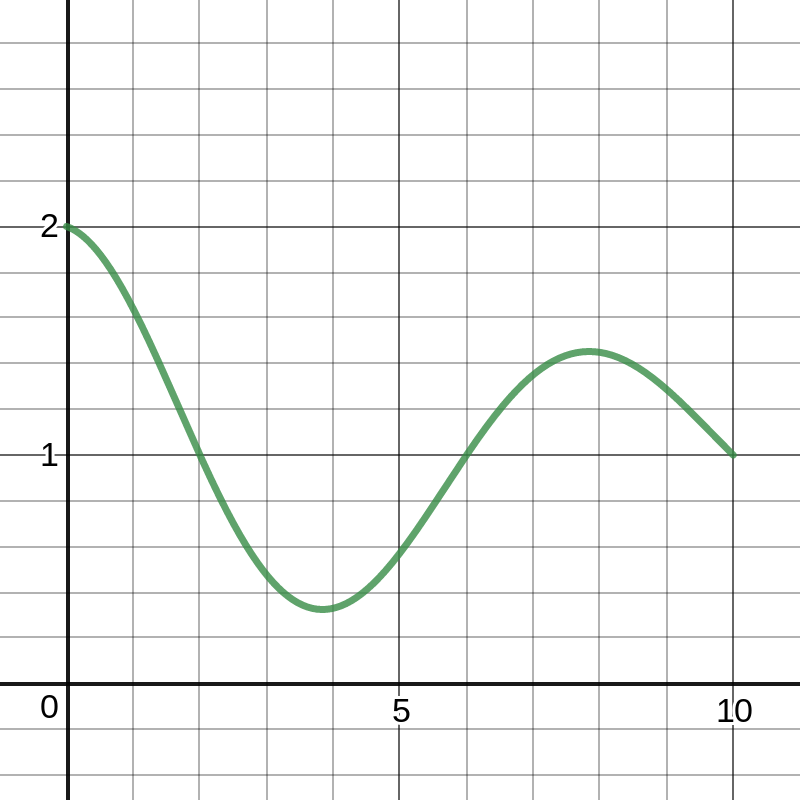
\includegraphics[width=3in]{ltc8-v2.png}
\end{center}
State the following points, intervals, and units. You may phrase your intervals using interval notation (for example, $[-1,2]$ is the set of all $x$-values between $-1$ and $2$, including the endpoints) or as inequalities (for example, $-1 \leq x \leq 2$). Note that in some of these questions, there could be more than one correct point or interval --- state all points or intervals that apply. 

\begin{enumerate}
    \item The interval(s) on which $f(x)$ is increasing
    \item The interval(s) on which $f'(x)$ is negative 
    \item The interval(s) on which $f''(x)$ is negative 
    \item The point(s) at which $f$ changes from concave up to concave down and vice versa
    \item The units of measurement of $f'(x)$
\end{enumerate}


\vfill


\begin{small}
    \begin{framed}
        	\textbf{Criteria for Satisfactory grade:} At least four answers out of five possible are correct (meaning that the given answers are correct and all applicable points or intervals are stated). 
    \end{framed}

\end{small}

\end{document}
